In this chapter, we will introduce some background knowledge about neural machine translation on three aspects,
namely, \textit{modeling}, \textit{training}, and \textit{decoding}

\section{Modeling}
We start from discussing the building blocks that forms the most recent Neural Machine Translation (NMT) models. 
For all different architectures, NMT can always be seen as a conditional language model. 
The introduction of the attention mechanism becomes the key which enables the NMT to achieve the state-of-the-art performance.

\subsection{Neural Language Modeling}
Before discussing the details of nerual machine translation, we first come to the general topic of generating sentence using neural networks, a.k.a. neural language modeling. The research of language modeling with neural networks dates back to \citep[NNLM, ][]{bengio2003neural}  where the authors used a feed-forward network to predict next words with a fixed window size of words as input. In general, when we consider the problem of natural language modeling, a simplified view is to model languages (e.g. sentences) in a generative framework: let $V$ the vocabulary of all possible tokens, for a sentence $Y=\{y_1, y_2, ..., y_T\}$, $y_t \in V$, the language model finds a set of parameters $\theta$ to represent the reconstruction probability
$p(Y;\theta)=p(y_1, y_2, ..., y_T; \theta)$.
\paragraph{Autoregressive Language Model} Directly modeling the probability of the entire sentence $Y$ is hard and intractable. Therefore aside from some research works, most of previous efforts reformulates the probability in an autoregressive way, that is,
\begin{equation}
\label{cp2.eq.autolm}
    p(Y;\theta) = \prod_{t=1}^{T+1}p(y_t|y_{0:t-1}; \theta),
\end{equation}
where special tokens $y_0$ (e.g. $\langle \mathrm{bos}\rangle$) and $y_{T+1}$ (e.g. $\langle \mathrm{eos}\rangle$) are used to represent the beginning and end of all target sentences. The intuiative view is that the language model shows that each generated tokens $y_t$ is conditional to all previous generated tokens.
% Note that, Eq.~\ref{cp2.eq.autolm} does not require any approximation.

\paragraph{Parameterization} 
We are interested in parameterizing (approximating) these conditional probabilities using neural networks, which can be feed-forward networks, convolutional networks, or recurrent neural networks~\citep[RNNLM, ][]{mikolov2010recurrent}. 
Take the RNNLM -- a generic formulation for language model -- as an example. For each time-step $t$, the whole history $y_{0: t-1}$ is summarized as:
\begin{equation}
    \begin{split}
         z_t = f(\epsilon_I[y_{t-1}], z_{t-1}; {\theta}_f) , t \in [1, T]
    \end{split}
\end{equation}
where $\epsilon_I$ is an embedding matrix and each row maps a fixed-length vector for each input words, $f$ is the recurrent networks used to summarize the history. In practise, instead of using the vanilla RNN, RNNs with gated units are often used to capture long-term dependency in language modeling, for instance, Long-short term memory~\citep[LSTM,][]{hochreiter1997long} or Gatetd Recurrent Units~\citep[GRU,][]{cho2014learning}.
Therefore, we can compute the output probability of $y_t$ by
\begin{equation}
    \label{cp2.eq.output}
    p(y_t|y_{0: t-1};\theta) = \mathop{\softmax}\limits_{y_t\in V}\left(\epsilon_O[y_t]\cdot z_t^T\right)
\end{equation}
where $\softmax(x) = \left. {e^x} \large / {\sum_{x'} e^{x'}} \right.$ is to ensure the probabilities sum to $1$, and $\epsilon_O$ is the output weights which are sometimes tied with $\epsilon_I$. More complicated structure with multiple layers of networks can be used to enhance the modeling ability.


%These conditional probabilities are parameterized using a neural network. Typically, an encoder-decoder architecture~\citep{sutskever2014sequence} with a unidirectional RNN-based decoder is used to capture the causal structure of the output distribution.

\subsection{Sequence-to-Sequence Learning}
The neural language modeling tells how likely to a natural language sentence can be generated from nowhere, which however, is not practical in real applications. In most cases, what we are interested in is to generate meaningful sentences with certain conditions, which includes not only machine translation -- the main focus of this thsis -- but many other tasks like summarization, captioning, question answering, and response generation in dialog system. Fortunately, it is easy to borrow the experience of language modeling by assuming a conditional language modeling. 
It is also known as sequence-to-sequence ($\sts$) learning when the conditioning inputs are also sequences, e.g. neural machine translation.

\paragraph{Neural Machine Translation as \sts Learning} 
Let us denote $X=\left\{ x_1, \ldots, x_{T'} \right\}$ and $Y=\left\{ y_1, \ldots, y_T \right\}$ to denote source and target sentences in machine translation, respectively. Similar to language modeling, neural machine translation models the target sentence given the source sentence as a conditional autoregressive language model:
\begin{equation}
	\label{cp2.eq.auto_sts}
    p(Y|X) =  \prod_{t=1}^{T+1}p(y_t|y_{0:t-1}, x_{1:T'}; \theta),
\end{equation}
We can use the same output function as Eq.~\ref{cp2.eq.output} for each probability where in \sts learning, and the hidden states $z_t$ summarizes both the decoded and the source words
\begin{equation}
    \label{cp2.eq.hidden_state}
    \begin{split}
         z_t = f^{\textsc{dec}}(\epsilon_I[y_{t-1}], z_{t-1}, c_t(x_{1:T'}); {\theta}_f), t \in [1, T+1]
    \end{split}
\end{equation}
where $c_t(x_{1:T'})$ is the context representation of the source sentence $X$. For instance, a simple implementation proposed in \newcite{cho2014learning,sutskever2014sequence} is to use another RNN to encode the source words into a series of vector representations $h_1, ..., h_{T'}$ as 
\begin{equation}
    \label{cp2.eq.rnn_encoder}
    h_\tau = f^{\textsc{enc}}\left(\epsilon_{E}[x_\tau], h_{\tau-1}; \theta_e\right),  \tau \in [1, T']
\end{equation}
where each source word $x_\tau$ is projected into a continuous embedding space with $\epsilon_{E}$. Then, it is possible to use the last state $h_{T'}$ as the context $c$ considering it has compressed all the information we need to get the correct translation.

Borrowing the concepts from information theory, we usually call the $ f^{\textsc{enc}}$ and $ f^{\textsc{dec}}$ in \sts learning as the encoder and decoder, respectively. Intuitively in NMT, we first encode the whole source sentence $X$ into a fixed length vector $c = h_{T'}$, and then we decode the translation from it.

\begin{figure}
    \centering
    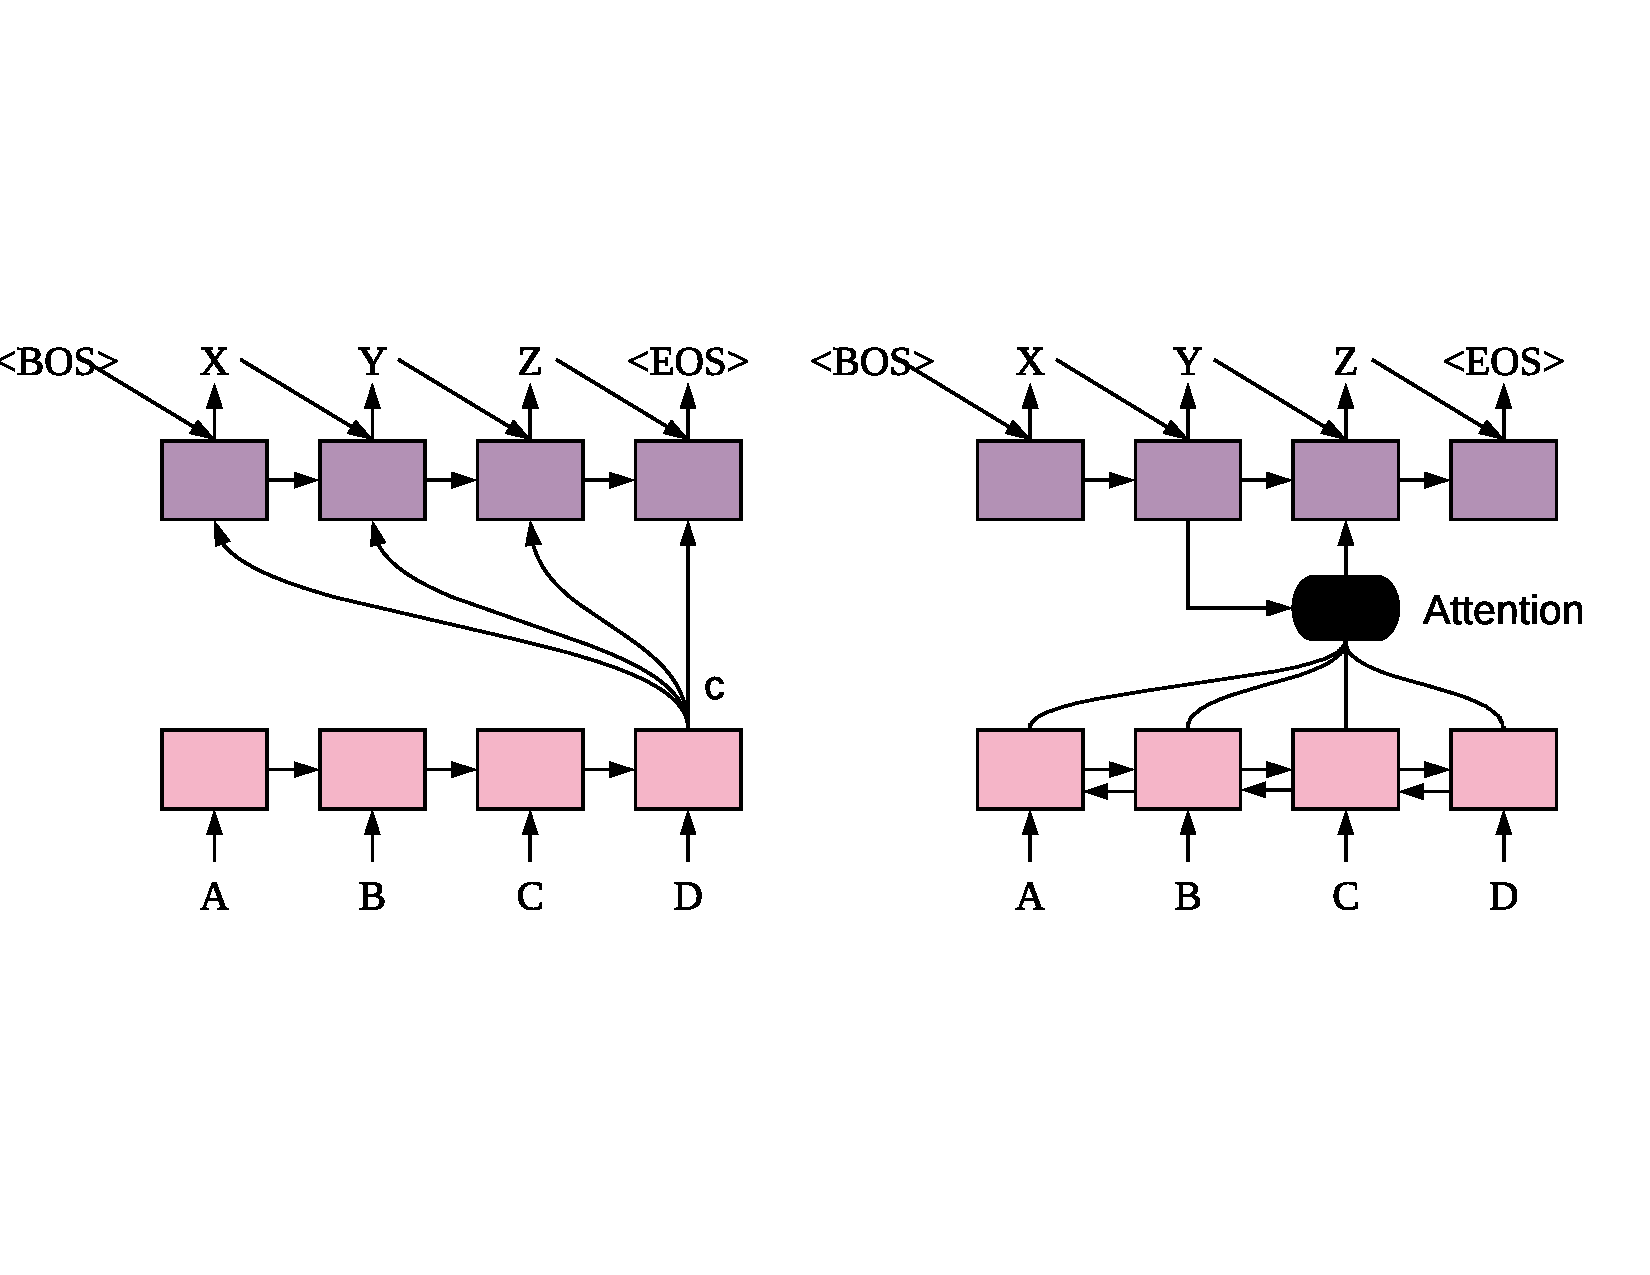
\includegraphics[width=\textwidth]{figs/background/s2s_att.pdf}
    \caption{An illustration of the comparison between the conventional \sts learning and \sts with attention mechanism for translating ``A B C D $\rightarrow$ X Y Z ''.}
    \label{cp2.fig.comparison}
\end{figure}

\subsection{Attention Mechanism}
Obviously, it is difficult to encode all the necessary information for translation into a fixed size vector, especially when the source sentence gets long. 
To release such burden, the attention mechanism was then introduced in~\newcite{bahdanau2014neural}, which was also inspired from the concept of ``alignment'' between source and target words in statistical machine translation. Instead of using a single vector for the whole decoding path, the attention mechanism uses a dynamically changing context $c_t$ in the decoding process. A natural option is to represent $c_t$ as the weighted sum of the source hidden states, i.e.
\begin{equation} 
    \label{cp2.eq.att}
	c_t = \sum_{\tau=1}^{T'}{\alpha_{t\tau} h_{\tau}}, \quad \alpha_{t\tau} =  \mathop{\softmax}\limits_\tau\left(f^{\textsc{att}}(z_{t-1}, h_{\tau}; \theta_a)\right),
\end{equation}
where $\alpha$ are the attention weights which is treated as soft-alignment, and $f^{\textsc{att}}$ is the function that shows the correspondence strength for attention, which can be either approximated with a multi-layer neural network or the inner-products between $z_{t-1}$ and $h_\tau$. 
Note that in~\newcite{bahdanau2014neural}, the source sentence is encoded with a bidirectional instead of an unidirectional RNN discussed above in Eq.~\ref{cp2.eq.rnn_encoder}, making each hidden state $h_{\tau}$ aware of the contextual information from both ends. 

The attention mechanism nicely solved the information compression problem in machine translation, and is the key for NMT to be able to achieve the state-of-the-art performance. See a comparison with a conventional \sts model in Fig.~\ref{cp2.fig.comparison}. For the following sections and chapters, without special notification, we in default consider the RNN-based \sts model with attention mechanism as the basic NMT model we used for exploration. 



\subsection{Neural Machine Translation without RNNs}
Since the entire target translation is known at training time (see more details in \S\ref{cp2.sec.mle}), the calculation of later conditional probabilities (and their corresponding losses) does not depend on the output words chosen during earlier decoding steps. 
Even though decoding must remain entirely sequential during inference, models can take advantage of this parallelism during training. Therefore, a trend of series of new approaches without RNN connections are quickly taking place the original RNN-based models.
For instance, such approaches replace RNNs in the decoder with parallelizable modules like  masked convolution~\cite{kalchbrenner2016neural, gehring2017convolutional} or self-attention (the Transformer)~\cite{vaswani2017attention}. A detailed illustration of the latter model is shown in Fig.~\ref{cp2.fig.transformer}. %that provide the causal structure required by the autoregressive factorization.
\begin{figure}[hptb]
	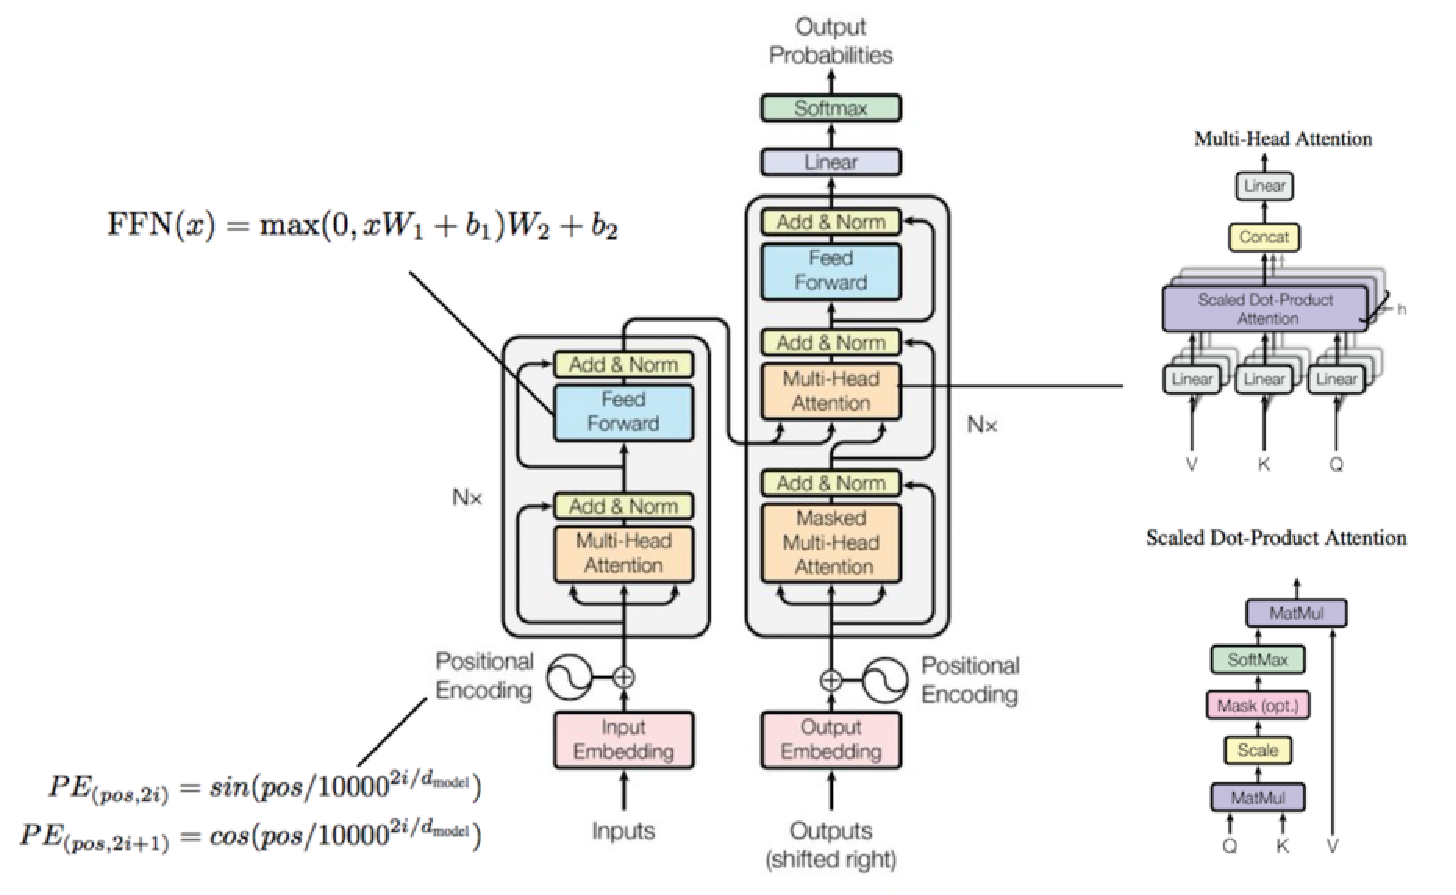
\includegraphics[width=\linewidth]{figs/background/transformer.pdf}
	\caption{\label{cp2.fig.transformer} A flow-chart of the Transformer model witch taken from \newcite{vaswani2017attention}. }
\end{figure}

%\paragraph{The Transformer Model}
%We specially introduce the Transformer model proposed in \newcite{vaswani2017attention} as an important example. 
%The Transformer model 
%A recently introduced option which reduces sequential computation still further is to construct the decoder layers out of self-attention computations that have been causally masked in an analogous way.
%The state-of-the-art Transformer network takes this approach, which allows information to flow in the decoder across arbitrarily long distances in a constant number of operations, asymptotically fewer than required by convolutional architectures \citep{vaswani2017attention}.

\section{Training}
\subsection{Data}
\paragraph{Parallel corpora} The training  of a typical NMT system requires large amount of parallel corpus, which is usually collected from bilingual documents done by human translators.  However, as we have already noted before, a typical NMT model usually requires millions of translated sentence pairs. 
%\paragraph{Monolingual corpora}
\paragraph{Vocabulary and Sub-word level translation}  
Training a standard NMT system usually needs a dictionary to store all the words which we normally call it the vocabulary. Typically, the size of the vocabulary has to be big (around $40,000$) so that it can generally assign embeddings for the majority of the words. If some words appear too rare to be calculated, a special symbol out-of-vocabulary (OOV) would be used as a replacement. 

To overcome the large vocabulary issue and the OOV problem to some extent, \newcite{sennrich2015neural} proposed to preprocess the training data by splitting rare words into pieces -- byte-pair-encoding (BPE) --  and then we run the NMT model at this sub-word level on both source and target sides. In general, the usage of BPE can normally increase the translation performance by $2$ BLEU scores compared to the word-level models. Moreover, research works such as \newcite{kim2016character,chung2016character,lee2016fully} keep one step further and model the translation directly in a character-level.

We will address the data problem in the later chapters.

\subsection{Maximum Likelihood Learning}
\label{cp2.sec.mle}
We train an NMT model, or equivalently estimate $\theta =\{\theta_f, \theta_e, \theta_a, \epsilon_E, \epsilon_I, \epsilon_O \}$, by maximizing the log-probability of the target translation $Y$ given a source sentence $X$. That is, we maximize the log-likelihood function:
\begin{equation}
	\label{cp2.eq.learning}
    \mathcal{L}^{\text{ML}}(\theta)  = \frac{1}{N} \sum_{n=1}^N \sum_{t=1}^{T_n+1} \log p(y_t^n| y_{0:t-1}^n, x_{1:T'}^n; \theta),
\end{equation}
given a training set consisting of $N$ parallel sentence pairs. One of the fascinate things about NMT and deep learning is that, once we got the formulation of a differentiable objectives, the whole model parameters -- no matter how complex you choose your model to be -- can be trained end-to-end using stochastic gradient decent (SGD) via back-propagtation~\cite{rumelhart1986learning}. In practise, we can use modified grandients outputted from an optimizer function, such as Adadelta~\cite{zeiler2012adadelta} or Adam~\cite{kingma2014adam} to achieve a faster convergence speed and better performance .

It is important to note that this maximum likelihood learning does not take into account how a trained model would be used. Rather, it is only concerned with learning a distribution over all possible translations. 

%\subsection{Advanced Learning Algorithms}
%. More advanced training algorithms for NMT have been proposed in recent years~\citep{wiseman2016sequence,shen2015minimum,bahdanau2016actor,ranzato2015sequence}.

%\subsection{Multilingual Training of Neural Machine Translation}

\section{Decoding}
Once the model is trained, either by maximum likelihood learning or by any other recently proposed algorithms above, we can let the model translate a given sentence by finding a translation that maximizes 
\begin{equation}
\hat{Y} = \argmax_{Y} \log p(Y|X; \theta) =\argmax_{y_1, ..., y_T}\sum_{t=1}^{T+1} \log p(y_t| y_{0:t-1}, x_{1:T'_n}; \theta),
\end{equation}
where $\theta=\{\theta_f, \theta_e, \theta_a, \epsilon_E, \epsilon_I, \epsilon_O \}$, $y_0 = \langle \mathrm{bos}\rangle$ and $y_{T+1} = \langle \mathrm{eos}\rangle$. This process is so-called \textit{decoding}, which is, however, computationally intractable as the number of possible solutions grows exponentially when the decoding length $T$ increases. Although the training algorithms ensure a good approximation for the translation distribution, it does not tell how to find the translation given the distribution function. It is a usual practice to resort to approximate decoding algorithms.

\subsection{Greedy Decoding}

One such approximate decoding algorithm is greedy decoding. In greedy decoding, we follow the conditional dependency path and pick the symbol with the highest conditional probability so far at each step. This is equivalent to picking the best symbol one at a time from left to right in conditional language modeling. A decoded translation of greedy decoding is $\hat{Y} = (\hat{y}_1, \ldots, \hat{y}_T)$, where
\begin{equation}
\hat{y}_t =  \argmax_{y \in V} \log p(y|\hat{y}_{0:t-1}, x_{1:T'}; \theta).
\end{equation}
Despite its preferable computational complexity $O(|V| \times T)$, greedy decoding has been over time found to be undesirably sub-optimal.% (see, e.g., \citep{cho2016noisy}.) 

\subsection{Beam Search}  
\label{cp2.sec.bs}
A better option to improve the translation quality is to perform beam search.
Unlike greedy decoding which keeps only a single hypothesis, beam search keeps $K (>1)$ hypotheses simultaneously during decoding. 
That is, at each time step $t$, beam search picks $K$ hypotheses with the highest scores from the cached $K$ prefix sequences (beam)\footnote{We assume for the initial step $t=0$, we only has one symbol $\mathcal{C}_0 = \{$ \bos $\}$}:
\begin{equation}
    \mathcal{C}_{t-1} = \{\tilde{y}_{0:t-1}^{(1)}, \tilde{y}_{0:t-1}^{(2)}, ..., \tilde{y}_{0:t-1}^{(K)} \}
\end{equation}
by evaluating the cumulative conditional probabilities of all candidate hypotheses to obtain the next round of sequences: 
\begin{equation}
     \mathcal{C}_{t} = \{\tilde{y}_{0:t}^{(1)}, \tilde{y}_{0:t}^{(2)}, ..., \tilde{y}_{0:t}^{(K)} \} =
     \mathop{\argsort^K}\limits_{y_t\in V, \\  y_{0:t-1}\in \mathcal{C}_{t-1}} \sum_{t'=0}^t\log p(y_{t'}|y_{0:t'-1}, x_{1:T'}; \theta).
\end{equation}
This process repeats until one or some of the hypotheses hits the end-of-sentence symbol (\eos). Each ended sequence $\tilde{Y}$ will be selected from the cache and in the meantime, the beam size decreases $K = K - 1$.
When all hypotheses terminate, it returns the best hypothesis from the chosen sequences $\tilde{Y}_1, ..., \tilde{Y}_K$ by a re-ranking function. For instance, a simple but effective way is to use the log-probability factored by the decoding length:
\begin{equation}
    \hat{Y} = \argmax_{\tilde{Y}_1, ..., \tilde{Y}_K} \left(\frac{1}{|Y|}\right)^\alpha\cdot\log p(Y|X; \theta),
\end{equation}
where we use $|Y|$ to show the number of tokens in the decoded sentence, and $\alpha \in [0, 1]$. When we selected $\alpha=1$, the re-ranking score is equivalent to a normalized log-likelihood, or so-called perplexity. In practise, we can choose $\alpha \approx 0.6$ which can greatly help to avoid generating too short sentences.

Despite its superior performance compared to greedy decoding, the computational complexity grows linearly w.r.t. the size of beam $K$, which makes it less preferable especially in the production environment.

\subsection{Noisy Parallel Decoding}
\label{cp2.sec.noisy}
Another alternative we can consider from is the noisy, parallel decoding (NPD) algorithm proposed in \newcite{cho2016noisy}. The main idea behind NPD algorithm is that a better translation with a higher log-probability may be found by injecting unstructured noise in the transition function of the decoder. That is,
\begin{equation}
z_t = f^{\textsc{dec}}(\epsilon_I[y_{t-1}], z_{t-1} + n_t, c_t(x_{1:T'}); \theta_f), t\in [1, T+1]
\end{equation}
where $n_t \sim \mathcal{N}(0, {\sigma_0^2} \large / {t^2})$ is the time-dependent noise. In practise, we can also other ways to inject randomness in the inner representation of the decoding process, and run greedy decoding based on the ``noisy'' inputs. 
NPD avoids potential degradation of translation quality by running such a noisy greedy decoding process multiple times in parallel. An important lesson of NPD algorithm is that there exists a decoding strategy with the asymptotically same computational complexity that results in a better translation quality, and that such a better translation can be found by manipulating the hidden state of the recurrent network. 


